\documentclass[a4paper,14pt]{article}
\usepackage{float}
\usepackage{extsizes}
\usepackage{amsmath}
\usepackage{amssymb}
\everymath{\displaystyle}
\usepackage{geometry}
\usepackage{fancyhdr}
\usepackage{multicol}
\usepackage{graphicx}
\usepackage[brazil]{babel}
\usepackage[shortlabels]{enumitem}
\usepackage{cancel}
\usepackage{textcomp}
\usepackage{array}
\usepackage{longtable}
\usepackage{booktabs}
\usepackage{float}   % Para usar o modificador [H]

\columnsep=2cm
\hoffset=0cm
\textwidth=8cm
\setlength{\columnseprule}{.1pt}
\setlength{\columnsep}{2cm}
\renewcommand{\headrulewidth}{0pt}
\geometry{top=1in, bottom=1in, left=0.7in, right=0.5in}

\pagestyle{fancy}
\fancyhf{}
\fancyfoot[C]{\thepage}

\begin{document}
	
	\noindent\textbf{6FMA34 - Matemática} 
	
	\begin{center}Utilizando sentenças equivalentes (Versão estudante)
	\end{center}
	
	\noindent\textbf{Nome:} \underline{\hspace{10cm}}
	\noindent\textbf{Data:} \underline{\hspace{4cm}}
	
	%\section*{Questões de Matemática}
	~ \\
    \begin{multicols}{2}
    	\noindent Se duas sentenças abertas são equivalentes (têm o mesmo conjunto verdade), podemos resolver a sentença aberta que julgarmos mais fácil. Por exemplo, para resolver $2x < 8$, podemos escrever $2x < 8 \Leftrightarrow x < 4$. \\
    	Quando sentenças abertas são ligadas com conectivos \textbf{ou} ($\lor$) ou \textbf{e} ($\land$), temos um sistema de sentenças abertas. Lembre-se de que duas sentenças unidas com o conectivo \textbf{ou} só são falsas se ambas forem falsas e que sentenças unidas com o conectivo \textbf{e} só são verdadeiras se ambas forem verdadeiras.
    	\noindent\textsubscript{~------------------------------------------------------------------------}
    	\begin{enumerate}
			\item Resolva as inequações no universo dos inteiros. Use equivalências se você achar necessário.
			\begin{enumerate}[a)]
				\item $-x < 2$ \\\\
				\item $-x > -4$ \\\\
				\item $-x \leq 0$ \\\\
				\item $-x > 0$ \\\\
				\item $-x \geq 1$ \\\\
				\item $-x \leq -6$ \\\\
			\end{enumerate}
			\item Resolva os sistemas no universo $U = \mathbb{Z}$.
			\begin{enumerate}[a)]
				\item $
				\begin{cases}
					x = 1 \\
					\text{e} \\
					x = 4	
				\end{cases}$ \\\\\\\\
				\item $
				\begin{cases}
					x = 1 \\
					\text{ou} \\
					x = 4	
				\end{cases}$ \\\\\\\\
				\item $
				\begin{cases}
					-x = 7 \\
					\text{e} \\
					x = -2	
				\end{cases}$ \\\\\\\\
				\item $
				\begin{cases}
					-x = 6 \\
					\text{ou} \\
					-x = -9	
				\end{cases}$ \\\\\\\\
				\item $
				\begin{cases}
					x \geq 1 \\
					\text{e} \\
					x \geq 4	
				\end{cases}$ \\\\\\\\
				\item $
				\begin{cases}
					x \leq 0 \\
					\text{ou} \\
					x > 0	
				\end{cases}$ \\\\\\\\
				\item $
				\begin{cases}
					x < -3 \\
					\text{e} \\
					x > -4	
				\end{cases}$ \\\\\\\\
				\item $
				\begin{cases}
					x = -3 \\
					\text{ou} \\
					x > 1	
				\end{cases}$ \\\\\\\\\\\\\\\\\\\\\\\\
			\end{enumerate}
			\textbf{Desafio olímpico} \\
			(OBMEP) Uma caixa contém somente bolas azuis, verdes e brancas. O número de bolas brancas é o dobro do número de bolas azuis. Se colocarmos 10 bolas azuis e retirarmos 10 bolas brancas, a caixa passará a conter o mesmo número de bolas de cada cor. Quantas bolas a caixa contém? \\
			a) 30 ~~~~~~ b) 40 ~~~~~~ c) 60 ~~~~~~~~~~ d) 80 ~~~~~~~~~ e) 90
			\newpage
			\item Resolva os sistemas em $U = \mathbb{Z}$.
			\begin{enumerate}[a)]
				\item $
				\begin{cases}
					x = 0 \\
					\text{ou} \\
					x = 2
				\end{cases}$ \\\\
				\item $
				\begin{cases}
					x = 0 \\
					\text{e} \\
					x = 2
				\end{cases}$ \\\\
				\item $
				\begin{cases}
					x < 5 \\
					\text{e} \\
					x > 4
				\end{cases}$ \\\\
				\item $
				\begin{cases}
					x < -2 \\
					\text{ou} \\
					x = 1
				\end{cases}$ \\\\
			\end{enumerate}
			\item Sendo $U = \mathbb{Z}$, encontre uma equação equivalente para cada uma das equações abaixo.
			\begin{enumerate}[a)]
				\item $4x = 8$ \\\\\\
				\item $x + x = 5$ \\\\\\
				\item $6x + 2 = 2 + 6$ \\\\\\
				\item $-x = 4$ \\
			\end{enumerate}
			\item Resolva os seguintes sistemas em $U = \mathbb{Z}$
			\begin{enumerate}[a)]
				\item $
				\begin{cases}
					x \neq 2 \\
					\text{ou} \\
					x \neq 5
				\end{cases}$ \\\\
				\item $
				\begin{cases}
					x = 7 \\
					\text{e} \\
					x \neq 0
				\end{cases}$ \\\\
				\item $
				\begin{cases}
					(x = 1 \text{ou} x = 4) \\
					\text{e} \\
					x \neq 1
				\end{cases}$ \\\\
				\item $
				\begin{cases}
					x = 3 \\
					\text{ou} \\
					x < -2
				\end{cases}$ \\\\
			\end{enumerate}
			\item Em cada item são marcados alguns números inteiros. Apresente uma equação ou inequação ou sistema que seja satisfeito apenas para esses pontos.
			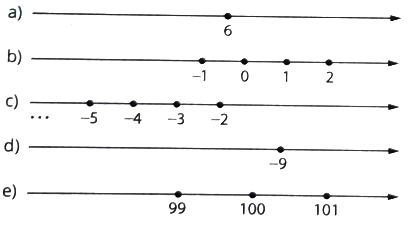
\includegraphics[width=1\linewidth]{imagens_6FMA34/imagem1}
			
    	\end{enumerate}
    $~$ \\ $~$ \\ $~$ \\ $~$ \\ $~$ \\ $~$ 
    \end{multicols}
\end{document}